\documentclass{article}
\usepackage{graphicx} % Required for inserting images
\usepackage{amsmath}
\usepackage{tikz}
\usetikzlibrary{shapes.multipart}


\title{ARBITRARY PRECISION ARITHMETIC}
\author{CS24BTECH11026}






\begin{document}

\maketitle


\section*{Introduction}

This project is about implementing an \textbf{arbitrary precision arithmetic} library in Java. The main goal is to implement accurate arithmetic operations on extremely large integers and floating point numbers without encountering overflow or round off errors which occurs generally. In programming, data types such as int or double have fixed sizes, which restrict the range and precision of numerical computations. To overcome these limitations, this project represents numbers as strings and implements arithmetic operations manually, allowing for complete control over precision and scale.
\newline

The library supports basic \textbf{operations addition, subtraction, multiplication, and division} for both integer and floating-point types. All operations are implemented in such a way that they preserve the full information of the numbers involved, avoiding any loss of precision due to rounding. For floating-point numbers, up to 30 digits of decimal precision are supported. and different ways to run this library by using python script and Ant make file.




\

\section*{Project Structure}
\begin{verbatim}
SDF_PROJECT/
      Java_files/                             
              arbitraryarithmetic/AFloat.java
                                  AInteger.java
      MyInfArith.java 
      arbitraryarithmetic/                    
                          aarithmetic.jar                  
      build/                                  
           arbitraryarithmetic/AInteger.class
                               AFloat.class
                               MyInfArith.class                        
      build.xml    
      PythonScript.py
      Report.tex
      
                            
\end{verbatim}

\section*{Integer Class(AInteger.java):}
AInteger class implements arbitrary precision for integers and implements methods for addition,subtraction,mutliplication and division even for large integers.

\subsection*{Constructors:}
\begin{itemize}
    \item Default constructor AInteger() that initializes the instance with value
0.
\item Constructor AInteger(String s) that initializes the instance by the
number whose string representation is given by ’s’. Eg: AInteger(“-
34534536454”);
\item Copy constructor that creates an instance of AInteger
\end{itemize}
\subsection*{Methods:}
Functions used to implement AInteger Class
\begin{itemize}

\item \textbf{public AInteger sub(AInteger s):} \\
Subtracts the given \texttt{AInteger} from the current instance and returns a new \texttt{AInteger} representing the result. Internally uses the \texttt{Sub} method on string values.

\item \textbf{public AInteger mul(AInteger s):} \\
Multiplies the current instance with the given \texttt{AInteger} and returns a new \texttt{AInteger} representing the product. Uses the \texttt{Multiply} method on string representations.

\item \textbf{public AInteger div(AInteger s):} \\
Divides the current instance by the given \texttt{AInteger} and returns a new \texttt{AInteger} representing the quotient. Relies on the \texttt{Division} method for computation.

\item \textbf{public int compare(String s1, String s2):} \\
Compares two non-negative integer strings \texttt{s1} and \texttt{s2}. Returns \texttt{1} if \texttt{s1 > s2}, \texttt{-1} if \texttt{s1 < s2}, and \texttt{0} if both are equal. It removes leading zeros before comparison.

\item \textbf{public String RemoveStartZero(String s):} \\
Removes leading zeros from the given string representation of a number. If the entire string is made of zeros, it returns \texttt{"0"}.

\item \textbf{public static AInteger parse(String s):} \\
A static method that takes a string \texttt{s} and returns a new \texttt{AInteger} instance initialized with that string.

\item \textbf{public AInteger(AInteger other):} \\
Copy constructor that creates a new \texttt{AInteger} with the same value as another \texttt{AInteger} instance.

\item \textbf{public AInteger(String s):} \\
Constructor that initializes an \texttt{AInteger} object with a string value representing a large integer.

\item \textbf{public AInteger():} \\
Default constructor that initializes the value to \texttt{"0"}.

\end{itemize}
\section*{UML Table(Integer class}
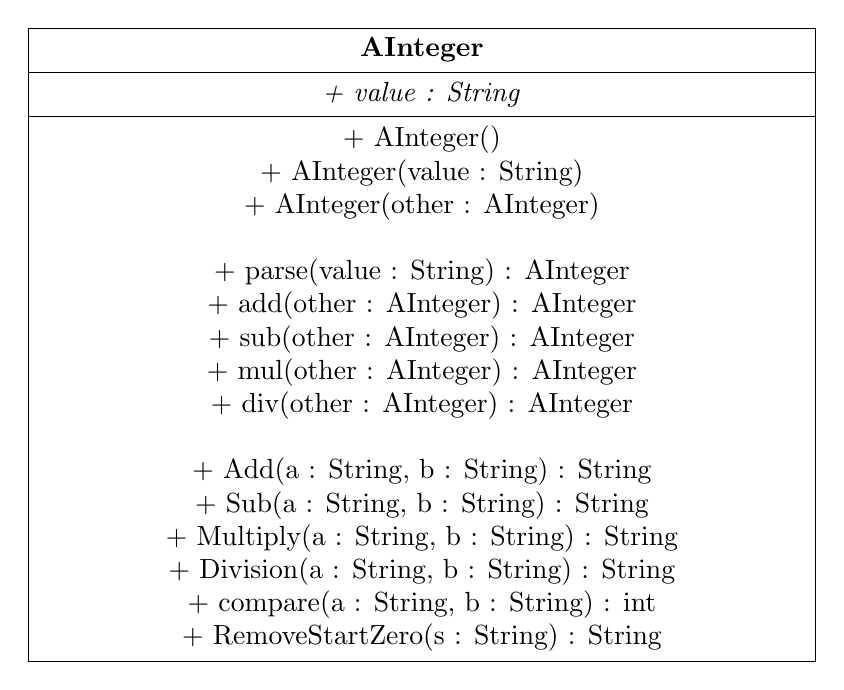
\begin{tikzpicture}
% Class Box for AInteger
\node[draw, rectangle split, rectangle split parts=3, minimum width=10cm, align=center, fill=white] (AInteger) {
    \textbf{AInteger} % Class Name
    \nodepart{second}
    \textit{+ value : String} % Attribute
    \nodepart{third}
    + AInteger()\\
    + AInteger(value : String)\\
    + AInteger(other : AInteger)\\
    \\
    + parse(value : String) : AInteger\\
    + add(other : AInteger) : AInteger\\
    + sub(other : AInteger) : AInteger\\
    + mul(other : AInteger) : AInteger\\
    + div(other : AInteger) : AInteger\\
    \\
    + Add(a : String, b : String) : String\\
    + Sub(a : String, b : String) : String\\
    + Multiply(a : String, b : String) : String\\
    + Division(a : String, b : String) : String\\
    + compare(a : String, b : String) : int\\
    + RemoveStartZero(s : String) : String
};

\end{tikzpicture}
\section*{Float Class(AFloat.java):}
AFloat class implements arbitrary precision for floating point numbers and implements methods for addition,subtraction,mutliplication and division even for large numbers with correct precision rounded off to 30 decimals after decimal point.

\begin{itemize}

\item \textbf{public AFloat add(AFloat s)} \\
Adds the given \texttt{AFloat} to the current instance and returns a new \texttt{AFloat} representing the result. Internally uses the \texttt{Add} method on string values.

\item \textbf{public AFloat sub(AFloat s)} \\
Subtracts the given \texttt{AFloat} from the current instance and returns a new \texttt{AFloat} representing the result. Internally uses the \texttt{Sub} method on string values.

\item \textbf{public AFloat mul(AFloat s)} \\
Multiplies the current instance with the given \texttt{AFloat} and returns a new \texttt{AFloat} representing the product. Uses the \texttt{Multiply} method on string representations.

\item \textbf{public AFloat div(AFloat s)} \\
Divides the current instance by the given \texttt{AFloat} and returns a new \texttt{AFloat} representing the quotient. Relies on the \texttt{Division} method for computation.

\item \textbf{public String Add(String Str1, String Str2)} \\
Adds two string representations of numbers and returns the result as a string.

\item \textbf{public String RemoveStartZero(String s)} \\
Removes leading zeros from the given string representation of a number. If the entire string is made of zeros, it returns \texttt{"0"}.

\item \textbf{public int compare(String Str1, String Str2)} \\
Compares two string representations of numbers numerically. Returns \texttt{1} if \texttt{Str1 > Str2}, \texttt{-1} if \texttt{Str1 < Str2}, and \texttt{0} if both are equal.

\item \textbf{public String Multiply(String Str1, String Str2)} \\
Multiplies two string representations of numbers and returns the result as a string.

\item \textbf{public String MultiplyF(String Str1, String Str2)} \\
Multiplies two floating-point string representations and returns the result as a string.

\item \textbf{public String Division(String Str1, String Str2)} \\
Divides two string representations of numbers and returns the quotient.

\item \textbf{public String RemoveEndZero(String Str)} \\
Removes trailing zeros from a string representation of a number with a decimal point.

\item \textbf{public String Sub(String Str1, String Str2)} \\
Subtracts two string representations of numbers and returns the result as a string.

\item \textbf{public String AddF(String Str1, String Str2)} \\
Adds two floating-point string representations and returns the result as a string.

\item \textbf{public String SubF(String Str1, String Str2)} \\
Subtracts two floating-point string representations and returns the result as a string.

\item \textbf{public String DivisionF(String Str1, String Str2)} \\
Divides two floating-point string representations and returns the result as a string.

\item \textbf{public String RoundOffTo30(String Str)} \\
Rounds a floating-point number represented as a string to 30 decimal places.

\item \textbf{public static AFloat parse(String s)} \\
A static method that takes a string \texttt{s} and returns a new \texttt{AFloat} instance initialized with that string.

\item \textbf{public AFloat(AFloat other)} \\
Copy constructor that creates a new \texttt{AFloat} with the same value as another \texttt{AFloat} instance.

\item \textbf{public AFloat(String s)} \\
Constructor that initializes an \texttt{AFloat} object with a string value representing a floating-point number.

\item \textbf{public AFloat()} \\
Default constructor that initializes the value to \texttt{"0.0"}.

\end{itemize}

\section*{UML Table(Float class):}
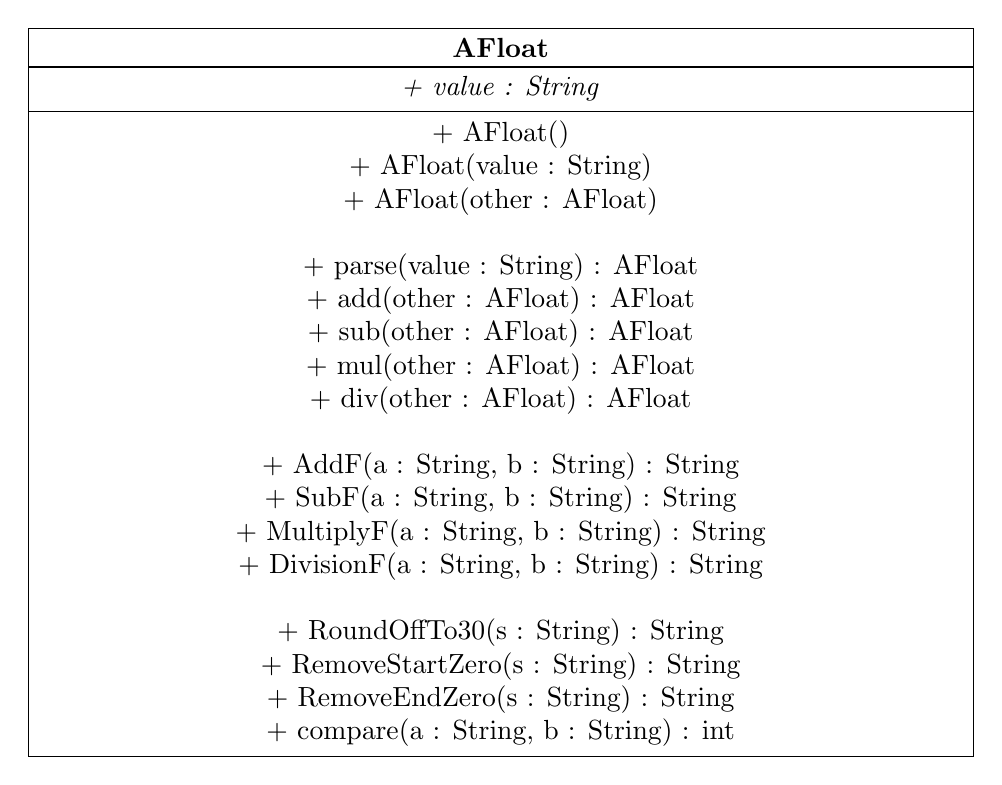
\begin{tikzpicture}
% Class Box for AFloat with white background
\node[draw, rectangle split, rectangle split parts=3, minimum width=12cm, align=center, fill=white] (AFloat) {
    \textbf{AFloat} % Class Name
    \nodepart{second}
    \textit{+ value : String} % Attribute
    \nodepart{third}
    + AFloat()\\
    + AFloat(value : String)\\
    + AFloat(other : AFloat)\\
    \\
    + parse(value : String) : AFloat\\
    + add(other : AFloat) : AFloat\\
    + sub(other : AFloat) : AFloat\\
    + mul(other : AFloat) : AFloat\\
    + div(other : AFloat) : AFloat\\
    \\
    + AddF(a : String, b : String) : String\\
    + SubF(a : String, b : String) : String\\
    + MultiplyF(a : String, b : String) : String\\
    + DivisionF(a : String, b : String) : String\\
    \\
    + RoundOffTo30(s : String) : String\\
    + RemoveStartZero(s : String) : String\\
    + RemoveEndZero(s : String) : String\\
    + compare(a : String, b : String) : int
};

\end{tikzpicture}
\section*{MyInfArith(Main file):}
MYInfArith is the main file to perform arithmetic operations .It takes input through 
command line arguements with supporting  four operations Addition,Subtraction,Multiplication and Division for both Integer and floating point numbers 
\section*{Input Format:}
Format: java MyInfArith $<type>$ $<operation>$ $<operand1>$ $<operand2>$
\subsection*{Arguements}


\begin{itemize}
  \item \textbf{$<type>$}: Specifies the data type for arithmetic.
  \begin{itemize}
    \item \texttt{"int"} – use \texttt{AInteger} class for operations on large integers.
    \item \texttt{"float"} – use \texttt{AFloat} class for operations on large floating-point numbers.
  \end{itemize}

  \item \textbf{$<operation>$}: The arithmetic operation to perform.
  \begin{itemize}
    \item \texttt{"add"} – addition
    \item \texttt{"sub"} – subtraction
    \item \texttt{"mul"} – multiplication
    \item \texttt{"div"} – division
  \end{itemize}

  \item \textbf{$<operand1>$}: The first number (as a string). Must be a valid integer or floating-point number depending on the type.

  \item \textbf{$<operand2>$}: The second number (as a string). Must be a valid integer or floating-point number depending on the type.
\end{itemize}



Based on the type given in arguements two objects(instances) are created using third and fourth arguements respectively, and performs the operation specified in the second arguement,prints the result as a string on screen if the number of digits after the decimal point exceeds 30,it will print upto 30 decimal points
\newline




\section*{Examples}

\begin{itemize}
  \item Integer addition:
  \begin{verbatim}
  java MyInfArith int add 123456789123456789 987654321987654321
  \end{verbatim}

  \item Floating-point multiplication:
  \begin{verbatim}
  java MyInfArith float mul 12345.6789 987.654321
  \end{verbatim}
\end{itemize}

\section*{Limitations of Library:}
\begin{itemize}
    \item For exytremely large numbers the multiplication and division operations takes time to give result because of manual digit by digit operation in methods
    \item It Supports only for four operations Addition,Subtraction,Division,Multiplication,does not support for higher operations like suqare,max,min functions
    \item Does not support for inputing scientific notation of large numbers and cannot handle other strings containg alphabets and different characters
    
\end{itemize}

\section*{Verification:}
\subsection*{Using Java:}
command: java MyInfArith $<type>$ $<operation>$ $<operand1>$ $<operand2>$
\begin{itemize}
    \item Ex:  Input: java MyInfArith int add 23650078224912949497310933240250
42939783262467113798386384401498 \\
Output: 66589861487380063295697317641748
   \item Ex:  Input: java MyInfArith int div 8792726365283060579833950521677211
493835253617089647454998358\\
Output: 17804979
\item Ex: Input: java MyInfArith float div 2.88832837283283 0.00000\\
Output: Exception in thread "main" java.lang.ArithmeticException: Division by Zero Error
\item Ex: Input: java MyInfArith float div 8792726365283060579833950521677211.0
493835253617089647454998358\\
Output: 17804979.091469989302961159520087878533

\end{itemize}
\subsection*{Using Python Script:}
command: python3 PythonScript.py $<type>$ $<operation>$ $<operand1>$ $<operand2>$ 
  (ubuntu)
\begin{itemize}
    \item Ex: Input:  python3 PythonScript.py float sub 840196454.51725 712586963.70283\\
    Output: 127609490.81442
    \item Ex: Input:  python3 PythonScript.py float mul 6400251.9377695 2326541.6827934\\
    Output: 14890452913599.9717457253213 
\end{itemize}
\subsection*{Using Ant:}
command: ant run -Darg1=$<type>$ -Darg2=$<operation>$ -Darg3=$<operand1>$ -Darg4=$<operand2>$
\begin{itemize}
    \item Ex: Input: ant run -Darg1=float -Darg2=div -Darg3=244727.15202 -Darg4=75964.3891  \\
    Output: 3.221603634537752111008551505615
    \item Ex: Input: ant run -Darg1=int -Darg2=div -Darg3=22 -Darg4=125\\
    Output: 0
\end{itemize}
\subsection*{Using Jar file:}
command: java -cp $Java_files:arbitraryarithmetic/aarithmetics.jar$ MyInfArith $<type>$ $<operation>$ $<operand1>$ $<operand2>$ 

\begin{itemize}
    


\item Ex: Input: java -cp $Java_files:arbitraryarithmetic/aarithmetic.jar$ 
 MyInfArith  int sub 3116511674006599806495512758577 57745
242300346381144446453884008\\
    Output: -54628730626339781337950941125431
    

\end{itemize}

\section*{Key Learnings:}

\begin{itemize}
    \item Java oops,creating packages
    \item Ant Make File
    \item Jar File
    \item Git commands and pushing into github
    \item Running Python script using os module 
    \item Docker 
\end{itemize}










  







    














\end{document}
